%----Rules for writing with Geoff
% 1. No second person, unless you are serious saying "this is what __we__ did. Rather use third
% person passive, e.g., instead of "we did this" use "this was done".
% 2. Start each sentence on a new line, to make it easy to reorder sentences.
% 3. Send me your BibTeX entries - I'll add them to the bibliography file in my standard format.
%----
\documentclass[runningheads]{llncs}

\usepackage[T1]{fontenc}
\usepackage{graphicx}
% \renewcommand\UrlFont{\color{blue}\rmfamily}
\usepackage{hyperref}
\usepackage{color}
\usepackage{setspace}
\usepackage{verbatim}
\usepackage{multicol}
\usepackage{array}
\usepackage{bbding}
\newcommand{\PreserveBackslash}[1]{\let\temp=\\#1\let\\=\temp}
\newcolumntype{C}[1]{>{\PreserveBackslash\centering}p{#1}}
\newcolumntype{R}[1]{>{\PreserveBackslash\raggedleft}p{#1}}
\newcolumntype{L}[1]{>{\PreserveBackslash\raggedright}p{#1}}
\setlength{\tabcolsep}{3pt}

%----Making things more compact
%----Suppress extra space in texttt mode
%\AddToHook{cmd/ttfamily/after}{\frenchspacing}
\renewcommand{\textfraction}{0.07}
\renewcommand{\topfraction}{0.9}
\renewcommand{\bottomfraction}{0.9}
\renewcommand{\floatpagefraction}{0.66}
\setlength{\floatsep}{2.0pt plus 2.0pt minus 2.0pt}
\setlength{\textfloatsep}{5.0pt plus 2.0pt minus 0.0pt}
\renewcommand{\textfloatsep}{2.0ex}
\renewcommand{\dbltextfloatsep}{2.0ex}

\newcommand{\proves}{{\footnotesize {\raisebox{0.3ex}{$\;\models$\;}}}}
\newcommand{\smalltt}[1]{\small \texttt{#1}}
\newenvironment{packed_itemize}{
\vspace*{-0.2em}
\begin{itemize}
\setlength{\partopsep}{0pt}
\setlength{\itemsep}{1pt}
\setlength{\parskip}{0pt}
\setlength{\parsep}{0pt}
}{\end{itemize}}
\newenvironment{packed_enumerate}{
\vspace*{-0.2em}
\begin{enumerate}
\setlength{\partopsep}{0pt}
\setlength{\itemsep}{1pt}
\setlength{\parskip}{0pt}
\setlength{\parsep}{0pt}
}{\end{enumerate}}

\begin{document}

\title{The TPTP Format for Tableaux Proofs}
\titlerunning{TPTP Tableaux}

\author{
Geoff Sutcliffe\inst{1}\orcidID{0000-0001-9120-3927}\Envelope
\and
\\ Sean B. Holden\inst{2}\orcidID{0000-0001-7979-1148}
\and
\\ Mantas Baksys\inst{2}\orcidID{0000-0001-9532-1007}
}
\authorrunning{Geoff Sutcliffe, et al.}
\institute{University of Miami, USA,
\email{geoff@cs.miami.edu},
\and
University of Cambridge, United Kingdom,
\email{sbh11@cl.cam.ac.uk,mb2412@cam.ac.uk}
}

\maketitle
%--------------------------------------------------------------------------------------------------
\begin{abstract}
Geoff

\keywords{Geoff}
\end{abstract}
%--------------------------------------------------------------------------------------------------
\section{Introduction}
\label{Introduction}

% Geoff

Automated Theorem Proving (ATP)~\cite{RV01-HAR} is concerned with the development and use of 
software that automates sound reasoning: the derivation of conclusions that follow inevitably 
from known facts.
ATP is at the heart of many computational tasks, including sensitive tasks such as 
software/hardware verification~\cite{HH19} and system security~\cite{Coo18}.
% New and emerging application areas include
% chemistry \cite{Yad17}, 
% biology \cite{CC+13}, 
% medicine \cite{HLB05},
% elections \cite{Nip09,BDS17}, 
% auctions \cite{CK+15}, 
% privacy \cite{Lib20},
% law \cite{PS15}, 
% ethics \cite{DF+16}, 
% religion \cite{OZ11,BW14-ECAI,Hor19},
% and business \cite{Han98}.
ATP systems are often used as components of more complex Artificial Intelligence (AI) systems,
which means that the impact of ATP extends into many facets of society.
% in areas such as 
% knowledge representation \cite{TR+04}, 
% natural language processing \cite{BM05}, 
% planning \cite{NV07}, 
% agents \cite{TBP03}, 
% commonsense reasoning \cite{MS05}, 
% and the semantic web \cite{McG04}.
In many of these applications the use of ATP systems is mission critical, in the sense that 
incorrect results from ATP might have nasty consequences.
% The importance of verifying the results from autonomous systems (including ATP systems) is
% reflected in the IEEE~P2817 standard, which aims to ``identify best practices and provide guidance 
% that supports the definition of valid verification processes for a range of autonomous system 
% configurations''.\footnote{%
% \href{https://standards.ieee.org/ieee/2817/11726/}{\smalltt standards.ieee.org/ieee/2817/11726/}}
Facing the demand for error-free results from ATP systems is the reality that ATP systems
are complex pieces of software, implementing complex calculi with complex data structures and
algorithms~\cite{Sch06}. 
Despite best intentions and efforts, incorrect results are possible.
% Two forms of incorrectness are most evident. 
% Firstly, an ATP system claiming to have found a solution when there is none, e.g., claiming to 
% have proved a non-theorem.
%MODEL or established the consistency of an unsatisfiable set of formulae. 
% Secondly, outputting a flawed solution, e.g., a proof that contains unsound inferences.
%MODEL or a model that has contradictory mappings for the symbols in the input problem.
To counter incorrectness, an ATP system can be required to output a proof
%MODEL solution, e.g., a proof or a model, which 
that serves as a certificate for the system's claim.
To ensure that a 
%MODEL solution 
proof is correct, proof verification can be required, 
which serves as a certification (but not a certificate) of the proof.
%MODEL solution.
% If the verifier outputs evidence for the certification in a form that can be independently 
% checked, that evidence serves as a certificate for the verifier's claim.
% As a concrete example, consider the verification process for aerospace software, shown in 
% Figure~\ref{NASACodeCertification}, taken from ~\cite{SDF05}.
% The ``proofs'' output by the ATP system are certificates that the ``safety policy'' has been 
% verified.  
% However, certification authorities like the FAA must be given explicit evidence that 
% the individual tool components (here, the ``ATP'' system) yield correct results.
% To that end the ATP system's proofs are given to a ``proof checker'' that produces certificates 
% that are attached to the ``code''.
%  
% \begin{figure}[htb]
% \begin{center}
% %EASYCHAIR 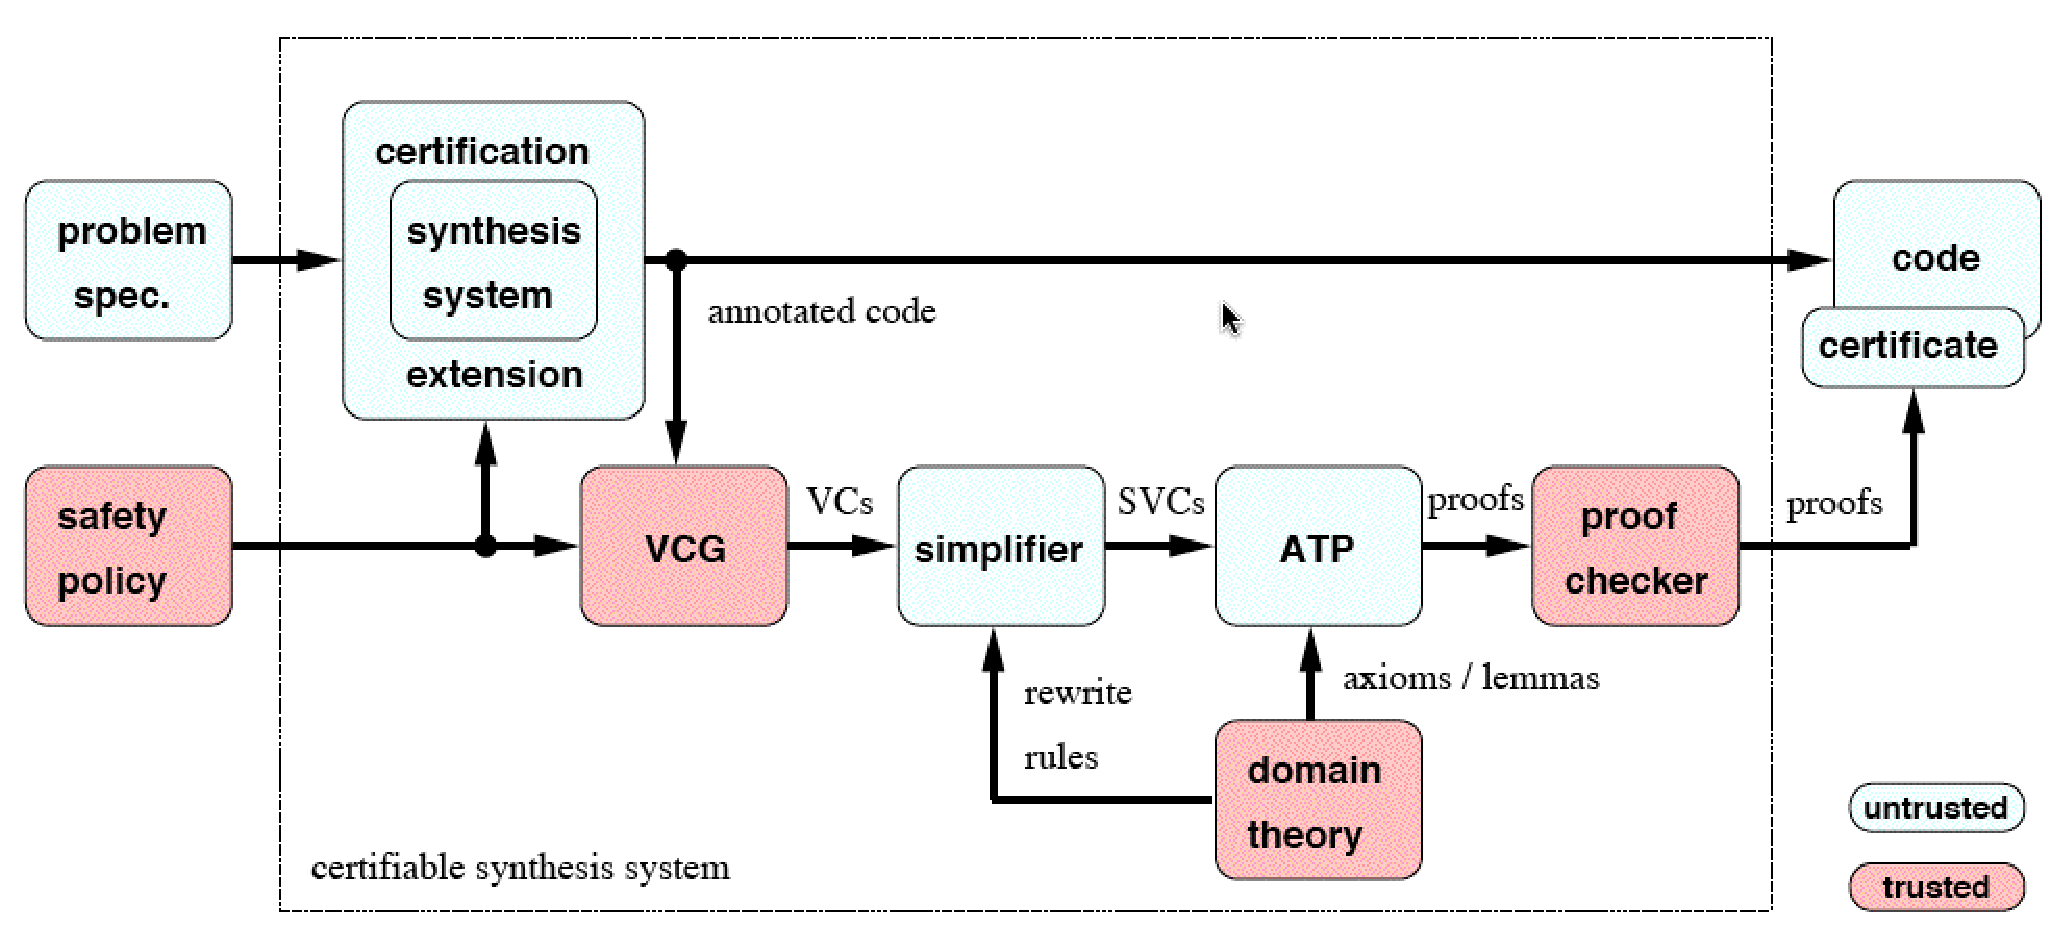
\includegraphics[width=0.6\textwidth]{NASACodeCertification}
% 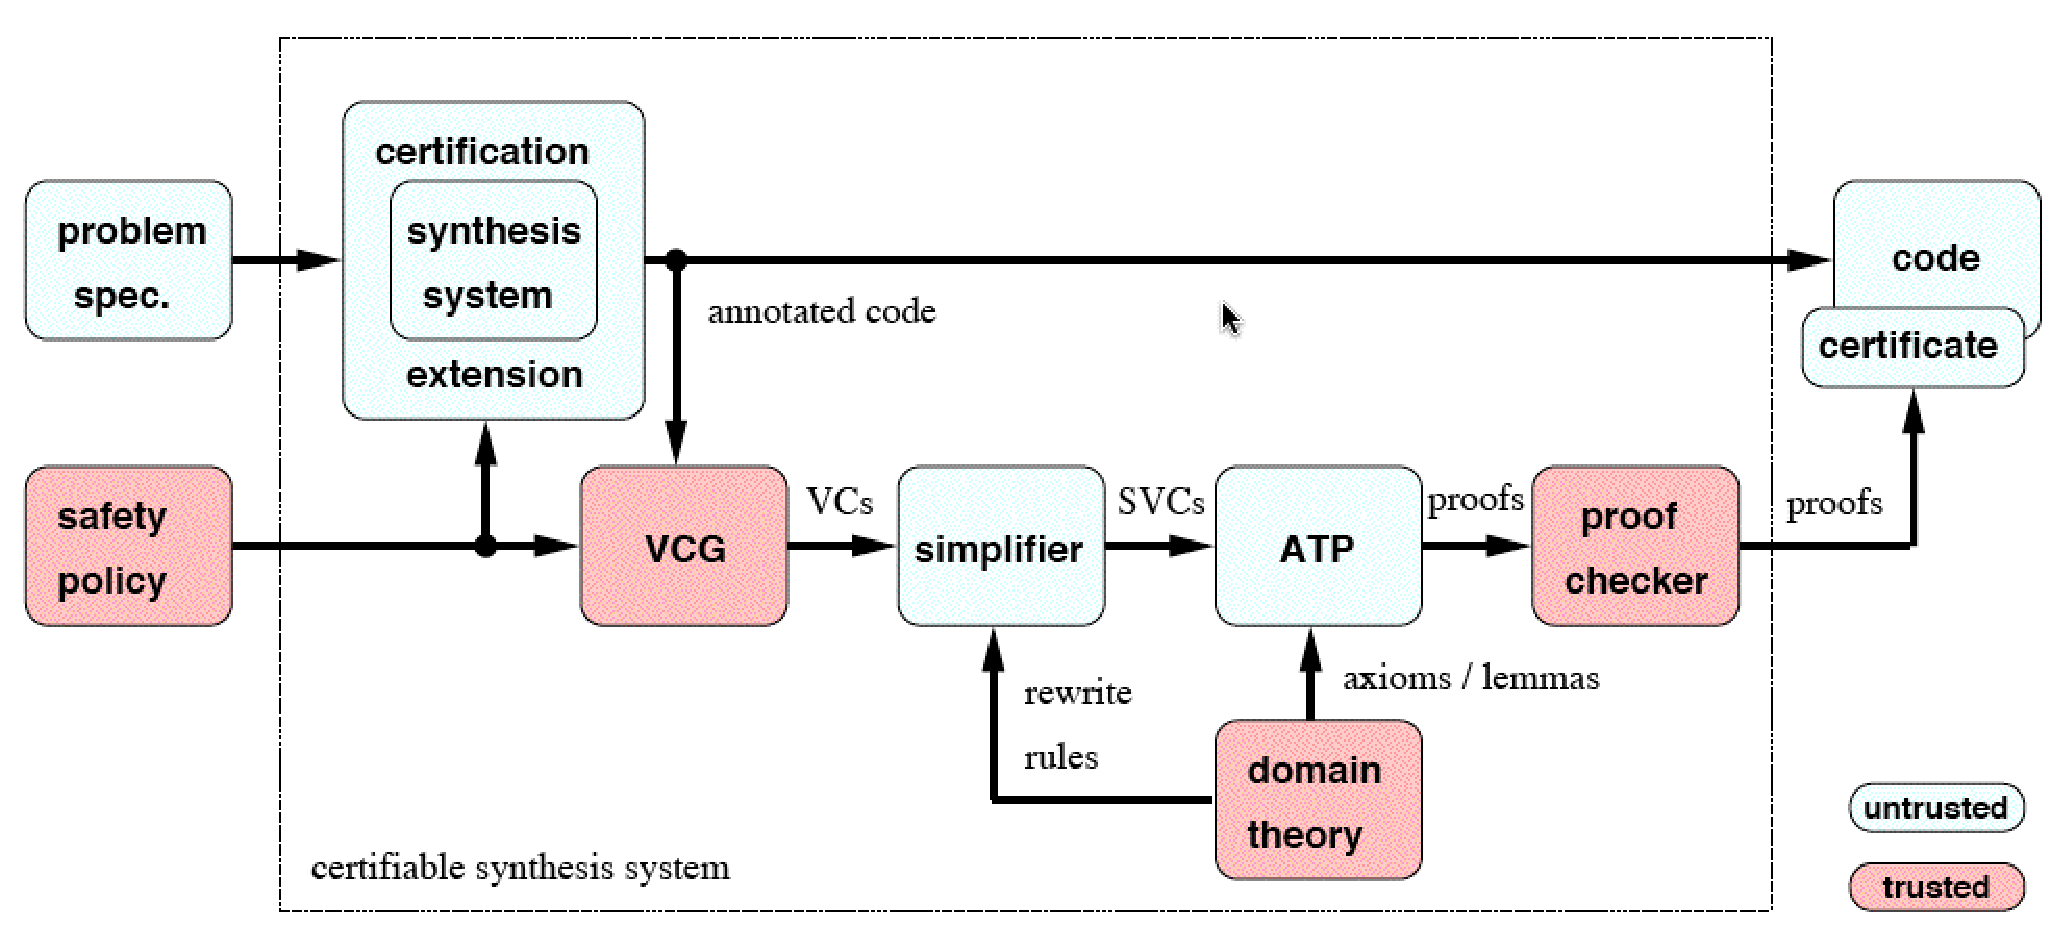
\includegraphics[width=0.8\columnwidth]{NASACodeCertification}   %FLAIRS
% \caption{Practical proof checking for program certification}
% \label{NASACodeCertification}
% \end{center}
% \end{figure}

At one top level, proofs can be divided into two types: Hilbert-style proofs that start at
axioms and derive theorems~\cite{End72}, and proofs-by-contradiction that negate the
conjecture to be proved and show that leads to a contradiction with the axioms~\cite{Men87}.
ATP systems that search for Hilbert-style proofs are often called ``natural deduction systems'',
e.g., THINKER~\cite{Pel98} and Muscadet~\cite{Pas01-IJCAR}.
Most contemporary high-performance ATP systems that search for a proof-by-contradiction, called
a refutation in this context, use a saturation based approach~\cite{Sch06}, e.g., E~\cite{SCV19} 
and Vampire~\cite{KV13}.
A complementary approach is taken in systems that build tableaux and closed connection 
matrices~\cite{FB+98}, e.g., leanCoP~\cite{Ott23} and Connect++~\cite{Hol23}.
The TPTP World (see Section~\ref{TPTP}) has an established format for writing Hilbert-style proofs 
and refutations~\cite{SS+06}, and has a tool for verifying proofs in that format (see
Section~\ref{Derivations}), but has not yet settled on a format for tableaux and connection
proofs.
One early proposal for a TPTP style format never gained traction~\cite{OS10}.
A more recent proposal~\cite{OH23} is in the TPTP style, and provided some inspiration for
the format proposed in this paper.

Sections~\ref{BLAH} provide ...
Section~\ref{Conclusion} concludes.

%--------------------------------------------------------------------------------------------------
\section{The TPTP World}
\label{TPTP}

% Geoff

The TPTP World~\cite{Sut24} is a well-established infrastructure that supports research, 
development, and deployment of Automated Theorem Proving (ATP) systems %(see 
%Section~\ref{TPTPWorld} for more details).
The TPTP World infrastructure includes
the TPTP language~\cite{SS+06},
the TPTP problem library~\cite{Sut09},
the TSTP solution library~\cite{Sut10},
the SZS ontologies~\cite{Sut08-KEAPPA},
the Specialist Problem Classes (SPCs) and problem difficulty ratings~\cite{SS01},
SystemOnTPTP~\cite{Sut00-CADE-17} and StarExec~\cite{SST14},
and the CADE ATP System Competition (CASC)~\cite{Sut16}.
The problem library is a large collection of Thousands of Problems for Theorem Proving -- hence 
the name. 
The problem library contains over 25000 problems from over 50 different domains, written in the 
TPTP language.
The problems are categorized into Specialist Problem Classes according to their syntactic and
logical status~\cite{Sut08-KEAPPA}.
The TSTP solution library is the result of running numerous ATP systems on that library and 
collecting their output. 
The solutions are categorized according to their logical and output form~\cite{Sut08-KEAPPA}.
The TPTP and TSTP libraries, with their categorizations, provide the basis for assigning a difficulty 
rating to each problem, according to the number of ATP systems that are able to solve 
it~\cite{SS01}.

The most salient feature of the TPTP World for this work is the TPTP language.
The TPTP language~\cite{Sut23-IGPL} is one of the keys to the success of the TPTP World.
The TPTP language is used for writing both problems and solutions,
which enables convenient communication between ATP systems and tools.
Originally the TPTP World supported only first-order clause normal form (CNF)
\cite{SS98-JAR}.
Over the years full first-order form (FOF)
\cite{Sut09}, 
typed first-order form (TFF)
\cite{SS+12,BP13-TFF1}, 
typed extended first-order form (TXF)
\cite{SK18}, 
typed higher-order form (THF)
\cite{SB10,KSR16}, 
and non-classical forms (NTF)~\cite{SF+22} have been added.
A general principle of the TPTP language is: ``We provide the syntax, you provide the semantics''.
As such, there is no a priori commitment to any semantics for each of the language forms, 
although in almost all cases the intended logic and semantics are well known.

Problems and solutions are built from {\em annotated formulae} of the form
\begin{center}
{\em language}{\tt (}{\em name}{\tt ,}
{\em role}{\tt ,}
{\em formula}{\tt ,}
{\em source}{\tt ,}
{\em useful\_info}{\tt )}
\end{center}
The {\em language}s supported are {\smalltt{cnf}} (clause normal form), {\smalltt{fof}}
(first-order form), {\smalltt{tff}} (typed first-order form), and {\smalltt{thf}}
(typed higher-order form).
The {\em role}, e.g., {\smalltt{axiom}}, {\smalltt{lemma}}, {\smalltt{conjecture}}, defines the 
use of the formula.
In a {\em formula}, terms and atoms follow Prolog conventions -- functions and predicates start 
with a lowercase letter or are {\tt '}single quoted{\tt '}, and variables start with an uppercase 
letter.
The language also supports interpreted symbols that either start with a {\tt \$}, e.g., the 
truth constants {\smalltt{\$true}} and {\smalltt{\$false}}, or are composed of 
non-alphabetic characters, e.g., integer/rational/real numbers such as 27, 43/92, -99.66.
The logical connectives in the TPTP language are
{\tt !>}, {\tt ?*}, {\tt @+}, {\tt @-}, {\tt !}, {\tt ?}, {\tt {\raisebox{0.4ex}{\texttildelow}}}, 
{\tt |}, {\tt \&}, {\tt =>}, {\tt <=}, {\tt <=>}, and {\tt <{\raisebox{0.4ex}{\texttildelow}}>},
for the mathematical connectives
$\Pi$, $\Sigma$, choice (indefinite description), definite description,
$\forall$, $\exists$, $\neg$, $\vee$, $\wedge$, $\Rightarrow$, $\Leftarrow$, $\Leftrightarrow$, 
and $\oplus$ respectively.
Equality and inequality are expressed as the infix operators {\tt =} and {\tt !=}.
The {\em source} and {\em useful\_info} are optional.
Figure~\ref{ExampleProblem} shows an example problem.

\begin{figure}[htb]
\centering
{\footnotesize
{\setlength{\baselineskip}{3mm}
\begin{verbatim}
%------------------------------------------------------------------------
fof(a1,axiom,         ~ ( ~ q(b) & ? [X] : s(X) ) ).

fof(a2,axiom,         ( r & q(b) ) => ! [X] : ~ p(X) ).

fof(a3,axiom,         p(c) | ! [Y] : ( ~ q(c) & q(Y) ) ).

fof(a4,axiom,         ~ q(c) => ~ q(b) ).

fof(a5,axiom,         p(c) => r ).

fof(prove,conjecture, ! [X] : ( ~ s(X) & ~ q(b) & p(c) ) ).
%------------------------------------------------------------------------
\end{verbatim}
}}
\caption{An example problem in TPTP format}
\label{ExampleProblem}
\end{figure}

%--------------------------------------------------------------------------------------------------
\subsection{The TPTP Format for Refutations}
\label{Derivations}

A refutation written in the TPTP language is a list of annotated formulae. 
The leaves of a refutation DAG are typically have a role {\smalltt axiom} or {\smalltt conjecture}, 
and the role for inferred formulae is typically one of {\smalltt negated\_conjecture} (also used 
for leaves in CNF) or {\smalltt plain} for inferred formulae. 
The source is either a {\smalltt file} record for leaves or an {\smalltt inference} record for 
inferred formulae.
A {\smalltt file} record contains the problem file name and the corresponding annotated formulae 
name in the problem file.
An {\smalltt inference} record contains the inference rule name, a list of useful inference 
information, and a list of the parent formulae.
The parent formulae list can contain parent annotated formulae names, and nested 
{\smalltt inference} records.
Common types of useful inference information are the semantic relationship of the inferred formula 
to its parents as an SZS ontology value~\cite{Sut08-KEAPPA} in a {\smalltt status} record, 
special information about recognized types of complex inference rules, e.g., Skolemization and
explicit splitting, and details of new symbols introduced in the inference.
The use of SZS values is core to GDV's approach to verification, described below.
The most common type of steps are those that infer a logical consequence of the parent formulae.
These are tagged with the SZS status {\smalltt{thm}}.
Another well known step is negating the conjecture, which is tagged with the SZS status 
{\smalltt{cth}}.
Steps of equi-satisfiability are tagged with the SZS status {\smalltt{esa}}. 

Figure~\ref{ExampleDerivation} shows an extract from the refutation found by E~3.2.5 for the
problem in Figure~\ref{ExampleProblem}.\footnote{%
The full refutation can be generated in \href{https://tptp.org/cgi-bin/SystemOnTPTP}{SystemOnTPTP}}
Points of note:
all the leaf formulae except {\tt a4} and {\tt a5} are copies of formulas in the problem;
{\tt a4} and {\tt a5} is easily derived from the corresponding problen formulae {\tt a5};
many of the formulae are inferred with SZS status {\smalltt{thm}}, i.e., they are logical 
consequences of their parents;
the negated conjecture {\smalltt c\_0\_7} is inferred with SZS status {\smalltt{cth}},
its negation is a logical consequence of its parent;
the inferred formulae, {\smalltt c\_0\_18} has a nested {\smalltt inference} record, and the 
intermediate inferred formula has not been recorded in the derivation. 

\begin{figure}[htb]
\centering
{\footnotesize
{\setlength{\baselineskip}{3mm}
\begin{verbatim}
%------------------------------------------------------------------------
%----Problem formulae in FOF (some ommitted)
fof(prove,conjecture,         ! [X1] : ( ~ s(X1) & ~ q(b) & p(c) ),
    file('PaperFOF.p',prove) ).

fof(a1,axiom,                 ~ ( ~ q(b) & ? [X1] : s(X1) ),
    file('PaperFOF.p',a1) ).

fof(a5,axiom,                 p(c) => r,
    file('PaperFOF.p',a5) ).

%----Clausification (some formulae omitted)
fof(c_0_6,negated_conjecture, ~ ! [X1] : ( ~ s(X1) & ~ q(b) & p(c) ),
    inference(assume_negation,[status(cth)],[prove]) ).

fof(c_0_11,negated_conjecture, s(esk1_0) | q(b) | ~ p(c),
    inference(skolemize,[status(esa)],[c_0_6]) ).

%----Refutation (some formulae omitted)
cnf(c_0_29,plain,              r | q(X1),
    inference(spm,[status(thm)],[c_0_25,c_0_27]) ).

cnf(c_0_30,plain,              r,
    inference(spm,[status(thm)],[c_0_28,c_0_29]) ).

cnf(c_0_31,plain,              ~ q(b),
    inference(cn,[status(thm)],
[inference(rw,[status(thm)],[c_0_23,c_0_30])]) ).

cnf(c_0_32,negated_conjecture, q(X1),
    inference(sr,[status(thm)],
[inference(spm,[status(thm)],[c_0_21,c_0_27]),c_0_31]) ).

cnf(c_0_33,plain,              $false,
    inference(cn,[status(thm)],
[inference(rw,[status(thm)],[c_0_31,c_0_32])]),
    [proof] ).
%------------------------------------------------------------------------
\end{verbatim}
}}
\caption{A extract from E 3.2.5's refutation of Figure~\ref{ExampleProblem}}
\label{ExampleDerivation}
\end{figure}

\begin{figure}[htb]
\centering
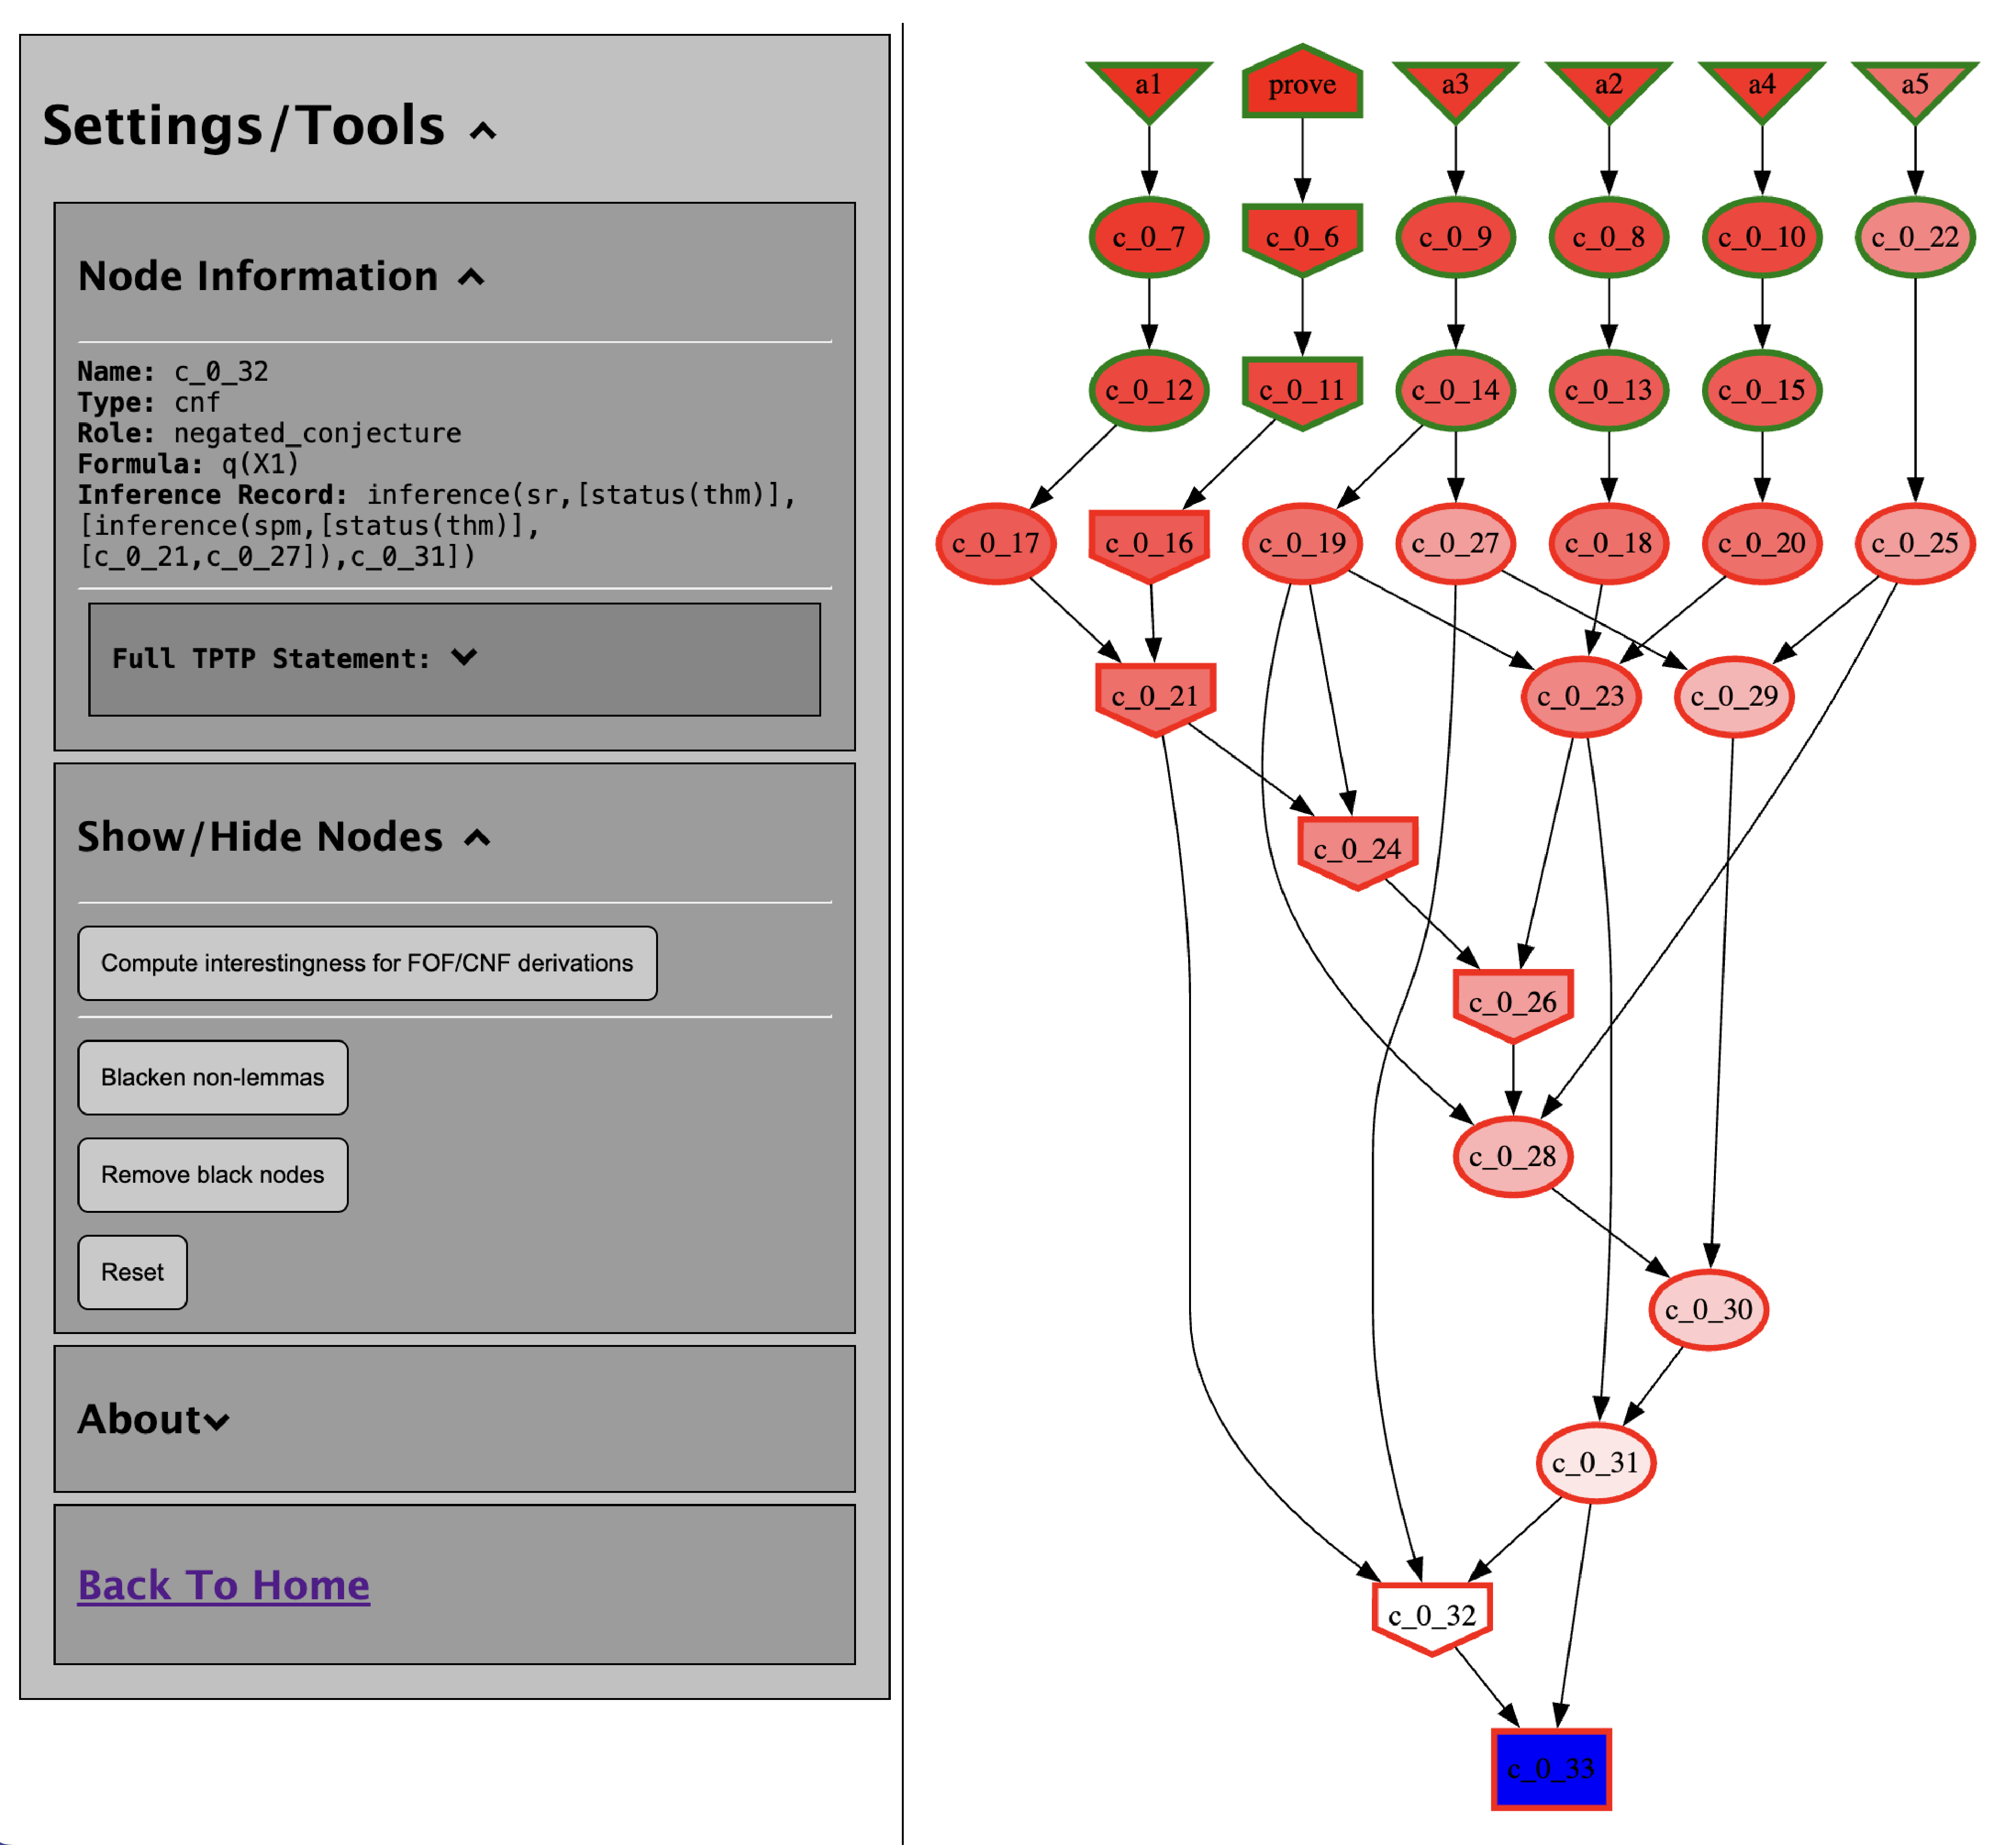
\includegraphics[width=0.8\textwidth]{PaperFOFIDV.pdf}
\vspace*{-1em}
\caption{Refutation extract for the problem in Figure~\ref{ExampleProblem}}
\label{Refutation}
\end{figure}

The GDV derivation verifier~\cite{Sut06} was developed at the start of the century, primarily
targeting proofs by refutation in clause normal and first-order form.
Over time it has been incrementally developed to verify proofs in typed first-order form and
typed higher-order form.
Most recently it has been developed to produce LambdaPi 
terms that can be independently verified using the {\smalltt lambdapi} checker.~\cite{SBB25}
GDV's input is a TPTP format refutation, and optionally (required for complete verification) the 
problem for which the proof was produced.
GDV checks a TPTP proof in four verification phases: structural verification, leaf verification,
rule-specific verification, and inference verification.
Many of the checks rely on a ``check-by-ATP'', which calls a trusted ATP system -- either a theorem 
prover or a model finder.
Structural verification deals with non-logical aspects of a proof, checking whether the
formulae presented as proof have the right format and relationships, e.g., all the parents of 
inferred formulae exist, the refutation is acyclic. 
Leaf verification deals with the leaves of the derivation, and their relationship with
the problem formulae, e.g., check-by-ATP that the leaf axioms are satisfiable, and that leaves 
are copies of problem formulae or can be proved from problem formulae using a check-by-ATP.
Rule specific verification deals with inference rules that require special treatment, e.g.,
explicit splitting~\cite{Wei01}, Skolemization. 
Inference verification deals with the various types of inferences that are made by ATP
systems in a proof.
Examples of checks are: for inference steps with SZS status {\smalltt{THM}} check-by-ATP that the 
inferred formula can be proved from the parent formulae, for inference steps with SZS status 
{\smalltt{CTH}} check-by-ATP that the negation of the inferred formula can be proved from the 
parent formulae.

% \begin{figure*}[htb]   %FLAIRS
% \begin{center}
% 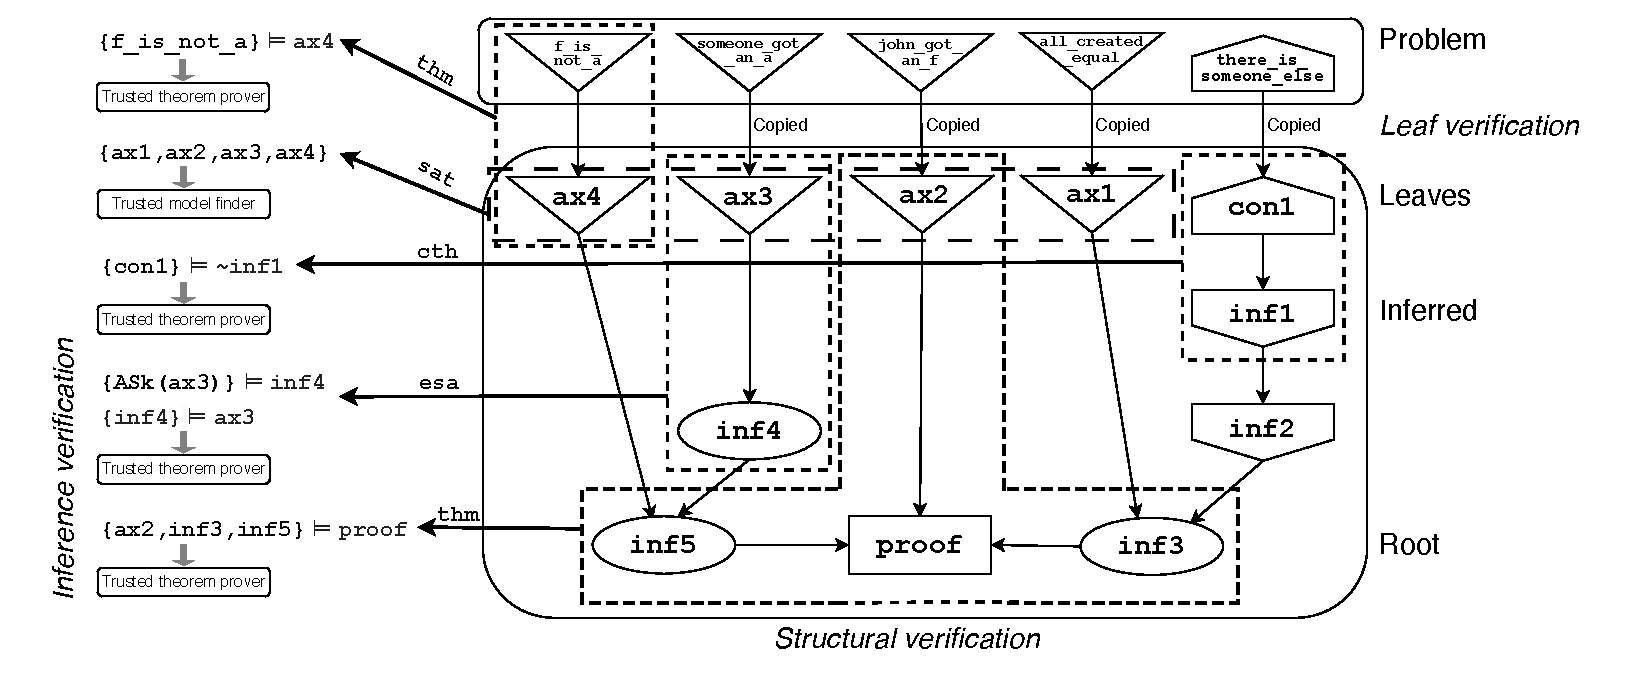
\includegraphics[width=1.0\textwidth]{GDVArchitecture}
% \caption{GDV architecture}
% \label{GDVArchitecture}
% \end{center}
% %EASYCHAIR \end{figure}
% \end{figure*}   %FLAIRS

The default trusted theorem provers and model finders used by GDV are Otter~\cite{McC03-Otter}
and E~\cite{SCV19} for theorem proving, Paradox~\cite{CS18}, Vampire~\cite{KV13}, and
Nitpick~\cite{BN10-ITP} for model finding.
These systems have become trusted through the process described in \cite{SBB25}.

%--------------------------------------------------------------------------------------------------
\section{The (new) TPTP Format for Tableau Proofs}
\label{Tableau}

Geoff: Requirements: semantic verification, tableau reconstruction.

Mantas: Explain the format, with two examples.
Note tableau has variables instantiated, if information is required {\tt bin()} records can be
added to the useful information list, e.g., 

\begin{verbatim}
cnf(t2,plain,              p(a),
    inference(extension,[status(thm),path([t1:1]),bind(t1:X,a)],[c3]) ).
\end{verbatim}

notes that the variable {\tt X} in the parent literal {\tt ~p(X)} gets bound to {\tt a}.
AAAARGH, WE NEED TO GET THIS VERY CLEAR.

\begin{figure}[htb]
\centering
{\scriptsize
{\setlength{\baselineskip}{3mm}
\begin{verbatim}
%--------------------------------------------------------------------------------------------
%----Problem formulae in FOF
fof(a1,axiom,              ~ ( ~ q(b) & ? [X] : s(X) ),           file('PaperFOF.p',a1) ).
fof(a2,axiom,              ( ( r & q(b) ) => ! [X] : ~ p(X) ),    file('PaperFOF.p',a2) ).
fof(a3,axiom,              ( p(c) | ! [Y] : ( ~ q(c) & q(Y) ) ),  file('PaperFOF.p',a3) ).
fof(a4,axiom,              ( ~ q(c) => ~ q(b) ),                  file('PaperFOF.p',a4) ).
fof(a5,axiom,              ( p(c) => r ),                         file('PaperFOF.p',a5) ).
fof(prove,conjecture,      ! [X] : ( ~ s(X) & ~ q(b) & p(c) ),    file('PaperFOF.p',prove) ).

%----Clausification
fof(nc1,negated_conjecture, ~ ! [X] : ( ~ s(X) & ~ q(b) & p(c) ),
    inference(negate,[status(cth)],[prove]) ).
fof(nc2,negated_conjecture, ? [X] : ~ ( ~ s(X) & ~ q(b) & p(c) ),
    inference(negate,[status(thm)],[nc1]) ).
fof(nc3,negated_conjecture, ~ ( ~ s(sK1) & ~ q(b) & p(c) ),
    inference(skolemize,[status(esq),new_symbols(skolem,[sK1]),skolemized(X)],[nc2]) ).
cnf(c1,plain,               ( q(b) | ~ s(X) ),
    inference(clausify,[status(thm)],[a1]) ).
cnf(c2,plain,               ( ~ q(b) | ~ p(X) | ~ r ),
    inference(clausify,[status(thm)],[a2]) ).
cnf(c3,plain,               ( p(c) | ~ q(c) ),
    inference(clausify,[status(thm)],[a3]) ).
cnf(c4,plain,               ( p(c) | q(Y) ),
    inference(clausify,[status(thm)],[a3]) ).
cnf(c5,plain,               ( q(c) | ~ q(b) ),
    inference(clausify,[status(thm)],[a4]) ).
cnf(c6,plain,               ( r | ~ p(c) ),
    inference(clausify,[status(thm)],[a5]) ).
cnf(c7,negated_conjecture,  ( s(sK1) | q(b) | ~ p(c) ),
    inference(clausify,[status(thm)],[nc3]) ).

%----Tableau
cnf(t1,plain,               ( q(b) | ~ s(X) ),
    inference(start,[status(thm),path([0:0])],[c1]) ).
cnf(t2,plain,               ( ~ q(b) | ~ p(X) | ~ r ),
    inference(extension,[status(thm),path([t1:1])],[c2]) ).
cnf(t3,plain,               $false,
    inference(connection,[status(thm),path([t2:1,t1:1])],[t2:1,t1:1]) ).
cnf(t4,plain,               ( p(c) | ~ q(c) ),
    inference(extension,[status(thm),path([t2:2,t1:1])],[c3]) ).
cnf(t5,plain,               $false,
    inference(connection,[status(thm),path([t4:1,t2:2,t1:1])],[t4:1,t2:2]) ).
cnf(t6,plain,               ( q(c) | ~ q(b) ),
    inference(extension,[status(thm),path([t2:2,t1:1])],[c5]) ).
cnf(t7,plain,               $false,
    inference(connection,[status(thm),path([t6:1,t4:2,t2:2,t1:1])],[t6:1,t4:2]) ).
cnf(t8,plain,               $false,
    inference(reduction,[status(thm),path([t6:2,t4:2,t2:2,t1:1])],[t6:2,t1:1]) ).
cnf(l1,plain,               p(c),
    inference(extension_lemma,[status(thm),path([t2:2,t1:1]),below(t1:1)],[t4:1]) ).
cnf(t9,plain,               ( r | ~ p(c) ),
    inference(extension,[status(thm),path([t2:3,t1:1])],[c6]) ).
cnf(t10,plain,              $false,
    inference(connection,[status(thm),path([t9:1,t2:3,t1:1])],[t9:1,t2:3]) ).
cnf(t11,plain,              $false,
    inference(lemma,[status(thm),path([l1:1,t9:2,t2:3,t1:1])],[l1:1,t9:2]) ).
cnf(l2,plain,               ~ q(b),
    inference(extension_lemma,[status(thm),path([t1:1]),below(0:0)],[t2:1]) ).
cnf(t12,plain,              ( s(sK1) | q(b) | ~ p(c) ),
    inference(extension,[status(thm),path([t1:2])],[c7]) ).
cnf(t13,plain,              $false,
    inference(connection,[status(thm),path([t12:1,t1:2])],[t12:1,t1:2]) ).
cnf(t14,plain,              $false,
    inference(lemma,[status(thm),path([l2:1,t12:2,t1:2])],[l2:1,t12:2]) ).
cnf(t15,plain,              ( p(c) | q(Y) ),
    inference(extension,[status(thm),path([t12:3,t1:2])],[c4]) ).
cnf(t16,plain,              $false,
    inference(connection,[status(thm),path([t15:1,t12:3,t1:2])],[t15:1,t2:3]) ).
cnf(t17,plain,              $false,
    inference(lemma,[status(thm),path([l2:1,t15:2,t12:3,t1:2])],[l2:1,t15:2]) ).
%--------------------------------------------------------------------------------------------
\end{verbatim}
}}
\caption{Full tableau in TPTP format}
\label{FullTableauCode}
\end{figure}

\begin{figure}[htb]
\centering
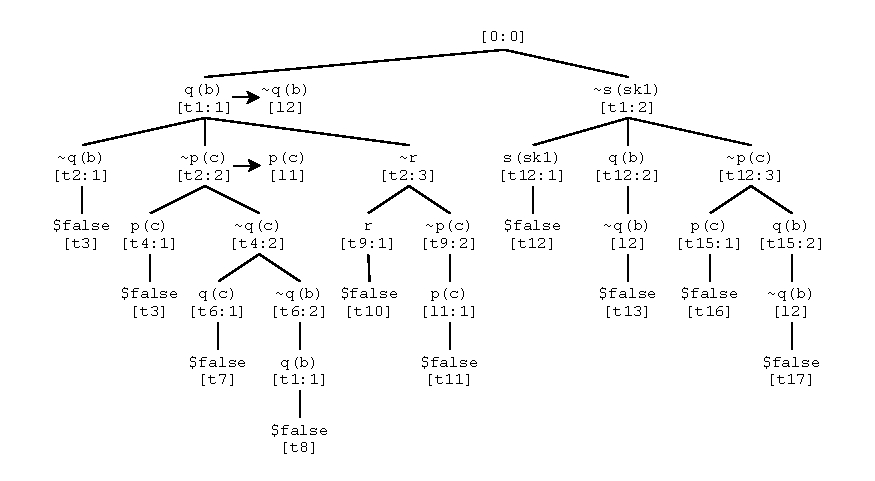
\includegraphics[width=0.8\textwidth]{Tableau.pdf}
\vspace*{-1em}
\caption{Tableau for the problem in Figure~\ref{ExampleProblem}}
\label{SimpleTableau}
\end{figure}

%--------------------------------------------------------------------------------------------------
\section{ATP Systems and Tools}
\label{SystemsTools}

Sean:
Connect++ and more.
Results from verifying a bunch of Connect++ tableau if we get the software done.

Geoff: GDV, IDV

%--------------------------------------------------------------------------------------------------
\section{Conclusion}
\label{Conclusion}

All.

%--------------------------------------------------------------------------------------------------
\bibliographystyle{splncs04}
\bibliography{Bibliography}
%--------------------------------------------------------------------------------------------------
\end{document}
